\documentclass[11pt,a4paper]{article}

\usepackage[margin=1in]{geometry}
\usepackage{amsmath,amssymb,mathtools}
\usepackage{bm}
\usepackage{enumitem}
\usepackage{tikz}
\usetikzlibrary{arrows.meta,calc,patterns,positioning,decorations.pathmorphing}
\usepackage{xcolor}
\usepackage{fancyhdr}
\usepackage{hyperref}
\usepackage{microtype}
\usepackage{booktabs}
\usepackage{array}
\usepackage{float}
\usepackage{caption}

\definecolor{navy}{HTML}{12324A}
\definecolor{teal}{HTML}{0F766E}
\definecolor{softteal}{HTML}{E7F6F4}
\definecolor{softblue}{HTML}{EEF5FF}
\definecolor{orange}{HTML}{C05621}
\definecolor{softorange}{HTML}{FFF3E8}
\definecolor{graytext}{HTML}{475569}
\definecolor{gridgray}{HTML}{CBD5E1}

\hypersetup{colorlinks=true, linkcolor=teal, urlcolor=teal}
\pagestyle{fancy}
\fancyhf{}
\lhead{Multivariable Calculus -- Problem Set 10}
\rhead{Detailed Solutions}
\cfoot{\thepage}
\renewcommand{\headrulewidth}{0.4pt}
\setlength{\parindent}{0pt}
\setlength{\parskip}{0.55em}
\setlength{\headheight}{14pt}
\setlist[enumerate]{leftmargin=2.1em, itemsep=0.35em}

% Lightweight breakable heading-style environments.
\newenvironment{methodbox}[1]{%
  \par\medskip
  \noindent\textcolor{navy}{\bfseries #1}\par
  \noindent\textcolor{navy}{\rule{\linewidth}{0.55pt}}\par\smallskip
}{\par\medskip}

\newenvironment{reasonbox}[1]{%
  \par\medskip
  \noindent\textcolor{teal}{\bfseries #1}\par
  \noindent\textcolor{teal}{\rule{0.72\linewidth}{0.45pt}}\par\smallskip
}{\par\medskip}

\newenvironment{answerbox}{%
  \par\medskip
  \noindent\textcolor{orange}{\rule{\linewidth}{0.8pt}}\par
  \begingroup\bfseries
}{%
  \par\endgroup
  \noindent\textcolor{orange}{\rule{\linewidth}{0.8pt}}\par\medskip
}

\newcommand{\R}{\mathbb{R}}
\newcommand{\dd}{\,d}
\newcommand{\pd}[2]{\frac{\partial #1}{\partial #2}}
\newcommand{\grad}{\nabla}
\newcommand{\curltest}{\frac{\partial Q}{\partial x}-\frac{\partial P}{\partial y}}

\begin{document}

\begin{center}
    {\Large\bfseries Problem Set 10: Detailed Assignment-Style Solutions}\\[0.35em]
    {\large Multivariable Calculus}\\[0.25em]
    {\small Lecturer: Rajendra Bhatia \quad TA: Debabrata Jana}
\end{center}

\begin{methodbox}{How this solution set is written}
Every computation is written in the same explicit pattern: first identify the relevant theorem, then compute the needed derivatives or parametrization, then substitute the limits, and finally state the exact value.  Diagrams are included where the geometry controls the calculation.  When a line integral is written as
\[
\int_C P(x,y)\,dx+Q(x,y)\,dy,
\]
the two scalar functions are always named as \(P\) and \(Q\) before applying any theorem.  This avoids hiding any step inside notation.
\end{methodbox}

\tableofcontents
\newpage

\section{Problem 1: Path independence and evaluation of line integrals}

\begin{methodbox}{General method for a plane line integral}
Suppose
\[
\int_C P(x,y)\,dx+Q(x,y)\,dy
\]
is given on a simply connected domain such as \(\R^2\).  The line integral is independent of path if the vector field
\[
F(x,y)=(P(x,y),Q(x,y))
\]
is conservative.  A practical test in the plane is:
\[
\pd{P}{y}=\pd{Q}{x}.
\]
If the test holds on all of \(\R^2\), then there is a potential function \(\phi\) such that
\[
\grad \phi=F.
\]
Then the Fundamental Theorem for Line Integrals gives
\[
\int_C P\,dx+Q\,dy=\phi(\text{end point})-\phi(\text{start point}).
\]
So the calculation reduces to finding \(\phi\) and evaluating it at the two endpoints.
\end{methodbox}

\begin{figure}[H]
\centering
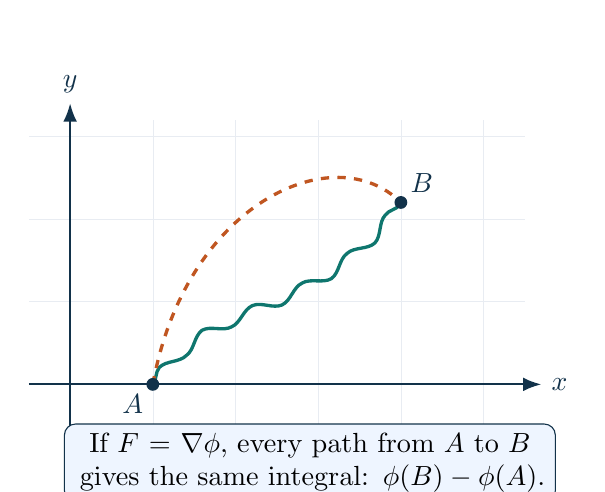
\begin{tikzpicture}[scale=1.05, >=Latex]
  \draw[step=1, gridgray!45, very thin] (-0.5,-0.5) grid (5.5,3.2);
  \draw[->, navy, thick] (-0.5,0) -- (5.7,0) node[right] {$x$};
  \draw[->, navy, thick] (0,-0.5) -- (0,3.4) node[above] {$y$};
  \coordinate (A) at (1,0);
  \coordinate (B) at (4,2.2);
  \draw[very thick, teal, decorate, decoration={snake, amplitude=0.7mm, segment length=7mm}] (A) .. controls (1.8,1.0) and (2.9,0.6) .. (B);
  \draw[very thick, orange, dashed] (A) .. controls (1.4,2.2) and (3.2,3.0) .. (B);
  \fill[navy] (A) circle (2.2pt) node[below left] {$A$};
  \fill[navy] (B) circle (2.2pt) node[above right] {$B$};
  \node[align=center, text width=6.0cm, fill=softblue, draw=navy, rounded corners] at (2.9,-0.95)
  {If $F=\nabla\phi$, every path from $A$ to $B$ gives the same integral: $\phi(B)-\phi(A)$.};
\end{tikzpicture}
\caption{Path independence means that only the endpoints matter, not the particular path.}
\end{figure}

\subsection{Problem 1(i)}
Evaluate
\[
\int_C 2xe^{-y}\,dx+\left(2y-x^2e^{-y}\right)\,dy,
\]
where \(C\) is any path from \((1,0)\) to \((2,1)\).

\begin{reasonbox}{Step 1: Identify the two component functions}
Compare the given integral with
\[
\int_C P\,dx+Q\,dy.
\]
Therefore
\[
P(x,y)=2xe^{-y},\qquad Q(x,y)=2y-x^2e^{-y}.
\]
\end{reasonbox}

\begin{reasonbox}{Step 2: Check whether the field is conservative}
Compute the two mixed partial derivatives required by the plane conservative-field test:
\[
\pd{P}{y}=\pd{}{y}\left(2xe^{-y}\right).
\]
The variable \(x\) is treated as a constant when differentiating with respect to \(y\). Since
\[
\pd{}{y}\left(e^{-y}\right)=-e^{-y},
\]
we get
\[
\pd{P}{y}=2x(-e^{-y})=-2xe^{-y}.
\]
Now compute
\[
\pd{Q}{x}=\pd{}{x}\left(2y-x^2e^{-y}\right).
\]
The term \(2y\) is constant with respect to \(x\), so its derivative is \(0\).  Also, \(e^{-y}\) is constant with respect to \(x\).  Hence
\[
\pd{Q}{x}=0-2xe^{-y}=-2xe^{-y}.
\]
Thus
\[
\pd{P}{y}=\pd{Q}{x}.
\]
Because the functions are smooth on all of \(\R^2\), the vector field is conservative on \(\R^2\).  Therefore the integral is independent of path.
\end{reasonbox}

\begin{reasonbox}{Step 3: Find a potential function}
We need \(\phi\) such that
\[
\pd{\phi}{x}=P=2xe^{-y},\qquad \pd{\phi}{y}=Q=2y-x^2e^{-y}.
\]
Start by integrating \(P\) with respect to \(x\):
\[
\phi(x,y)=\int 2xe^{-y}\,dx.
\]
Since \(e^{-y}\) is constant with respect to \(x\),
\[
\phi(x,y)=e^{-y}\int 2x\,dx=x^2e^{-y}+h(y).
\]
The extra term \(h(y)\) appears because differentiating with respect to \(x\) would erase any function depending only on \(y\).

Now differentiate this expression with respect to \(y\):
\[
\pd{\phi}{y}=\pd{}{y}\left(x^2e^{-y}+h(y)\right)=-x^2e^{-y}+h'(y).
\]
This must equal \(Q\), so
\[
-x^2e^{-y}+h'(y)=2y-x^2e^{-y}.
\]
Cancel \(-x^2e^{-y}\) from both sides:
\[
h'(y)=2y.
\]
Integrating gives
\[
h(y)=y^2+C.
\]
The constant does not affect the gradient, so we take \(C=0\). Therefore a potential function is
\[
\phi(x,y)=x^2e^{-y}+y^2.
\]
\end{reasonbox}

\begin{reasonbox}{Step 4: Evaluate by endpoints}
The starting point is
\[
A=(1,0),
\]
and the endpoint is
\[
B=(2,1).
\]
By the Fundamental Theorem for Line Integrals,
\[
\int_C 2xe^{-y}\,dx+\left(2y-x^2e^{-y}\right)\,dy=\phi(B)-\phi(A).
\]
Compute the endpoint values:
\[
\phi(2,1)=2^2e^{-1}+1^2=\frac{4}{e}+1,
\]
and
\[
\phi(1,0)=1^2e^0+0^2=1.
\]
Therefore
\[
\phi(2,1)-\phi(1,0)=\left(\frac{4}{e}+1\right)-1=\frac{4}{e}.
\]
\end{reasonbox}

\begin{answerbox}
The line integral is independent of path, and its value is
\[
\boxed{\frac{4}{e}}.
\]
\end{answerbox}

\subsection{Problem 1(ii)}
Evaluate
\[
\int_C \sin y\,dx+\left(x\cos y-\sin y\right)\,dy,
\]
where \(C\) is any path from \((2,0)\) to \((1,\pi)\).

\begin{reasonbox}{Step 1: Identify the two component functions}
Here
\[
P(x,y)=\sin y,
\qquad
Q(x,y)=x\cos y-\sin y.
\]
\end{reasonbox}

\begin{reasonbox}{Step 2: Check the conservative-field condition}
Compute
\[
\pd{P}{y}=\pd{}{y}(\sin y)=\cos y.
\]
Compute
\[
\pd{Q}{x}=\pd{}{x}(x\cos y-\sin y).
\]
The term \(\cos y\) is constant with respect to \(x\), so
\[
\pd{}{x}(x\cos y)=\cos y.
\]
The term \(-\sin y\) is independent of \(x\), so its \(x\)-derivative is \(0\). Therefore
\[
\pd{Q}{x}=\cos y.
\]
Hence
\[
\pd{P}{y}=\pd{Q}{x}.
\]
Since the field is smooth on all of \(\R^2\), it is conservative on \(\R^2\). Therefore the integral is independent of path.
\end{reasonbox}

\begin{reasonbox}{Step 3: Find a potential function}
We need \(\phi\) satisfying
\[
\pd{\phi}{x}=\sin y.
\]
Integrate with respect to \(x\):
\[
\phi(x,y)=\int \sin y\,dx=x\sin y+h(y).
\]
Now differentiate with respect to \(y\):
\[
\pd{\phi}{y}=x\cos y+h'(y).
\]
This must equal \(Q=x\cos y-\sin y\). Therefore
\[
x\cos y+h'(y)=x\cos y-\sin y.
\]
Cancel \(x\cos y\):
\[
h'(y)=-\sin y.
\]
Since
\[
\frac{d}{dy}(\cos y)=-\sin y,
\]
we may take
\[
h(y)=\cos y.
\]
Thus
\[
\phi(x,y)=x\sin y+\cos y.
\]
\end{reasonbox}

\begin{reasonbox}{Step 4: Evaluate by endpoints}
The start point is
\[
A=(2,0),
\]
and the end point is
\[
B=(1,\pi).
\]
Hence
\[
\int_C \sin y\,dx+\left(x\cos y-\sin y\right)\,dy=\phi(1,\pi)-\phi(2,0).
\]
Compute
\[
\phi(1,\pi)=1\cdot\sin \pi+\cos\pi=0-1=-1.
\]
Compute
\[
\phi(2,0)=2\cdot\sin 0+\cos0=0+1=1.
\]
Therefore
\[
\phi(1,\pi)-\phi(2,0)=-1-1=-2.
\]
\end{reasonbox}

\begin{answerbox}
The line integral is independent of path, and its value is
\[
\boxed{-2}.
\]
\end{answerbox}

\newpage
\section{Problem 2: The vector field on the punctured plane}

Consider the vector field on \(\R^2\setminus\{(0,0)\}\):
\[
F(x,y)=\left(\frac{-y}{x^2+y^2},\frac{x}{x^2+y^2}\right).
\]
We evaluate its line integral on two positively oriented circles centered at the origin.

\begin{methodbox}{General method for a circle centered at the origin}
A circle of radius \(a>0\), traced anticlockwise, is parametrized by
\[
\mathbf r(t)=(a\cos t,a\sin t),\qquad 0\leq t\leq 2\pi.
\]
Its derivative is
\[
\mathbf r'(t)=(-a\sin t,a\cos t).
\]
The line integral of a vector field \(F\) over this curve is
\[
\int_C F\cdot d\mathbf r=\int_0^{2\pi}F(\mathbf r(t))\cdot \mathbf r'(t)\,dt.
\]
This method is direct and does not require path independence.
\end{methodbox}

\begin{figure}[H]
\centering
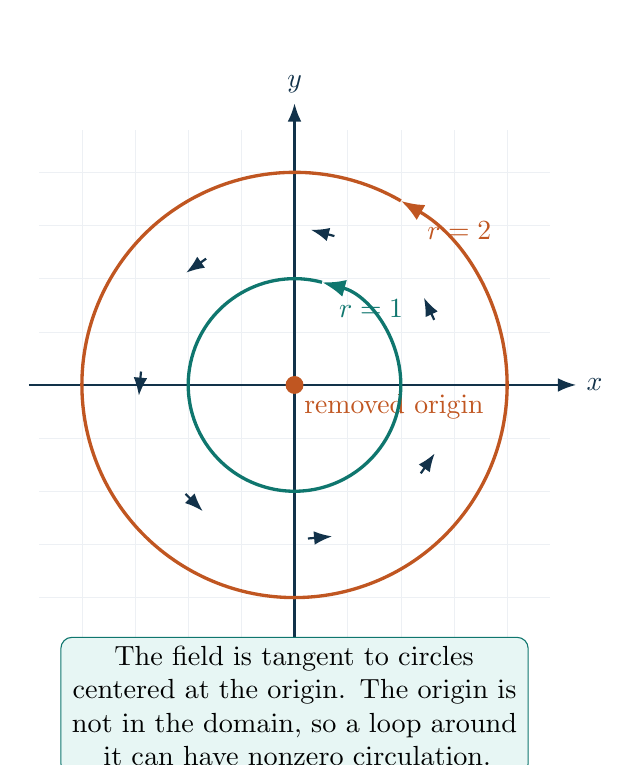
\begin{tikzpicture}[scale=1.35, >=Latex]
  \draw[step=0.5, gridgray!35, very thin] (-2.4,-2.4) grid (2.4,2.4);
  \draw[->, navy, thick] (-2.5,0) -- (2.65,0) node[right] {$x$};
  \draw[->, navy, thick] (0,-2.5) -- (0,2.65) node[above] {$y$};
  \fill[orange] (0,0) circle (2.4pt) node[below right] {removed origin};
  \draw[very thick, teal, ->] (1,0) arc (0:75:1);
  \draw[very thick, teal] (75:1) arc (75:360:1);
  \draw[very thick, orange, ->] (2,0) arc (0:60:2);
  \draw[very thick, orange] (60:2) arc (60:360:2);
  \node[teal] at (0.72,0.72) {$r=1$};
  \node[orange] at (1.55,1.45) {$r=2$};
  \foreach \ang in {25,75,125,175,225,275,325}{
    \pgfmathsetmacro{\x}{1.45*cos(\ang)}
    \pgfmathsetmacro{\y}{1.45*sin(\ang)}
    \pgfmathsetmacro{\tx}{-0.23*sin(\ang)}
    \pgfmathsetmacro{\ty}{0.23*cos(\ang)}
    \draw[->, navy, thick] (\x,\y) -- ++(\tx,\ty);
  }
  \node[align=center, text width=5.7cm, fill=softteal, draw=teal, rounded corners] at (0,-3.02)
  {The field is tangent to circles centered at the origin. The origin is not in the domain, so a loop around it can have nonzero circulation.};
\end{tikzpicture}
\caption{The vector field \(F=(-y/(x^2+y^2),x/(x^2+y^2))\) winds around the removed origin.}
\end{figure}

\subsection{Problem 2(i): Circle of radius 1}
Let
\[
C: \mathbf r(t)=(\cos t,\sin t),\qquad 0\leq t\leq 2\pi.
\]
Then
\[
\mathbf r'(t)=(-\sin t,\cos t).
\]
On this circle,
\[
x=\cos t,
\qquad
 y=\sin t,
\qquad
x^2+y^2=\cos^2t+\sin^2t=1.
\]
Therefore
\[
F(\mathbf r(t))=\bigl(-\sin t,\cos t\bigr).
\]
Now compute the dot product:
\[
F(\mathbf r(t))\cdot\mathbf r'(t)=(-\sin t,\cos t)\cdot(-\sin t,\cos t).
\]
Using the dot product formula,
\[
F(\mathbf r(t))\cdot\mathbf r'(t)=\sin^2t+\cos^2t=1.
\]
Hence
\[
\int_C F\cdot d\mathbf r=\int_0^{2\pi}1\,dt=2\pi.
\]

\begin{answerbox}
For the anticlockwise circle of radius \(1\),
\[
\boxed{\int_C F\cdot d\mathbf r=2\pi}.
\]
\end{answerbox}

\subsection{Problem 2(ii): Circle of radius 2}
Let
\[
C: \mathbf r(t)=(2\cos t,2\sin t),\qquad 0\leq t\leq 2\pi.
\]
Then
\[
\mathbf r'(t)=(-2\sin t,2\cos t).
\]
On this circle,
\[
x=2\cos t,
\qquad
 y=2\sin t,
\qquad
x^2+y^2=4\cos^2t+4\sin^2t=4.
\]
Therefore
\[
F(\mathbf r(t))=\left(\frac{-2\sin t}{4},\frac{2\cos t}{4}\right)=\left(-\frac12\sin t,\frac12\cos t\right).
\]
Now compute the dot product:
\[
F(\mathbf r(t))\cdot\mathbf r'(t)=\left(-\frac12\sin t,\frac12\cos t\right)\cdot(-2\sin t,2\cos t).
\]
Therefore
\[
F(\mathbf r(t))\cdot\mathbf r'(t)=\sin^2t+\cos^2t=1.
\]
Hence
\[
\int_C F\cdot d\mathbf r=\int_0^{2\pi}1\,dt=2\pi.
\]

\begin{answerbox}
For the anticlockwise circle of radius \(2\),
\[
\boxed{\int_C F\cdot d\mathbf r=2\pi}.
\]
\end{answerbox}

\begin{reasonbox}{Important conclusion}
Both circles give the same value \(2\pi\).  This does not mean the field is conservative on \(\R^2\setminus\{(0,0)\}\).  In fact, a conservative field has zero integral over every closed curve.  Since these closed circles have integral \(2\pi\neq0\), the field is not conservative on the punctured plane.
\end{reasonbox}

\newpage
\section{Problem 3: Green's Theorem}

\begin{methodbox}{Green's Theorem: calculation template}
For a positively oriented, simple closed curve \(C\) bounding a plane region \(R\), Green's Theorem says
\[
\oint_C P\,dx+Q\,dy
=\iint_R\left(\pd{Q}{x}-\pd{P}{y}\right)dA.
\]
The required steps are:
\begin{enumerate}
    \item identify \(P\) and \(Q\),
    \item compute \(\pd{Q}{x}-\pd{P}{y}\),
    \item describe the region \(R\) with explicit integral limits,
    \item evaluate the double integral.
\end{enumerate}
Positive orientation means counterclockwise orientation around the boundary.
\end{methodbox}

\subsection{Problem 3(i): Triangle}
Evaluate
\[
\oint_C xy^2\,dx+2x^2y\,dy,
\]
where \(C\) is the positively oriented triangle with vertices
\[
(0,0),\qquad (2,2),\qquad (2,4).
\]

\begin{figure}[H]
\centering
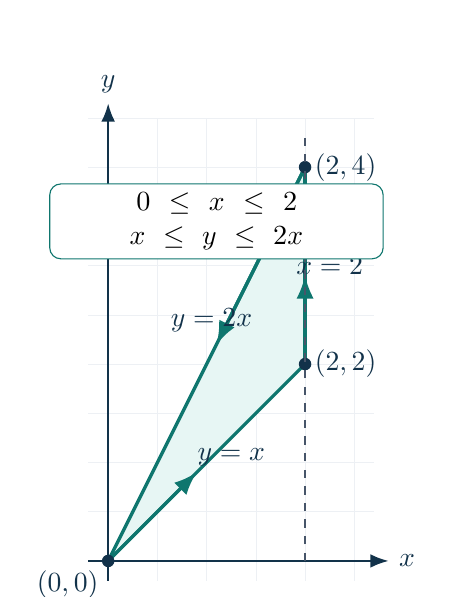
\begin{tikzpicture}[scale=1.25, >=Latex]
  \draw[step=0.5, gridgray!35, very thin] (-0.2,-0.2) grid (2.7,4.5);
  \draw[->, navy, thick] (-0.2,0) -- (2.85,0) node[right] {$x$};
  \draw[->, navy, thick] (0,-0.2) -- (0,4.65) node[above] {$y$};
  \coordinate (O) at (0,0);
  \coordinate (A) at (2,2);
  \coordinate (B) at (2,4);
  \fill[softteal] (O)--(A)--(B)--cycle;
  \draw[teal, very thick, ->] (O) -- ($(A)!0.55!(O)$);
  \draw[teal, very thick] (O) -- (A);
  \draw[teal, very thick, ->] (A) -- ($(B)!0.55!(A)$);
  \draw[teal, very thick] (A) -- (B);
  \draw[teal, very thick, ->] (B) -- ($(O)!0.55!(B)$);
  \draw[teal, very thick] (B) -- (O);
  \fill[navy] (O) circle (1.8pt) node[below left] {$(0,0)$};
  \fill[navy] (A) circle (1.8pt) node[right] {$(2,2)$};
  \fill[navy] (B) circle (1.8pt) node[right] {$(2,4)$};
  \node[navy] at (1.25,1.05) {$y=x$};
  \node[navy] at (1.05,2.45) {$y=2x$};
  \node[navy] at (2.25,3.0) {$x=2$};
  \draw[dashed, graytext] (2,0) -- (2,4.35);
  \node[align=center, fill=white, draw=teal, rounded corners, text width=4cm] at (1.1,3.45)
  {$0\le x\le2$\\ $x\le y\le2x$};
\end{tikzpicture}
\caption{The triangular region is described most simply by vertical slices: \(0\le x\le2\), \(x\le y\le2x\).}
\end{figure}

\begin{reasonbox}{Step 1: Identify \(P\) and \(Q\)}
Here
\[
P(x,y)=xy^2,
\qquad
Q(x,y)=2x^2y.
\]
\end{reasonbox}

\begin{reasonbox}{Step 2: Compute Green's Theorem integrand}
First compute
\[
\pd{Q}{x}=\pd{}{x}(2x^2y)=4xy.
\]
Next compute
\[
\pd{P}{y}=\pd{}{y}(xy^2)=2xy.
\]
Therefore
\[
\pd{Q}{x}-\pd{P}{y}=4xy-2xy=2xy.
\]
\end{reasonbox}

\begin{reasonbox}{Step 3: Describe the region}
The triangle has boundary lines:
\[
y=x,
\qquad
 y=2x,
\qquad
 x=2.
\]
For vertical slices, \(x\) starts at \(0\) and ends at \(2\).  For a fixed \(x\), \(y\) starts on the lower line \(y=x\) and ends on the upper line \(y=2x\).  Thus
\[
0\le x\le2,
\qquad
x\le y\le2x.
\]
\end{reasonbox}

\begin{reasonbox}{Step 4: Evaluate the double integral}
By Green's Theorem,
\[
\oint_C xy^2\,dx+2x^2y\,dy
=\iint_R 2xy\,dA.
\]
Using the limits above,
\[
\iint_R 2xy\,dA=\int_0^2\int_x^{2x}2xy\,dy\,dx.
\]
For the inner integral, \(x\) is constant:
\[
\int_x^{2x}2xy\,dy=2x\int_x^{2x}y\,dy.
\]
Now
\[
\int y\,dy=\frac{y^2}{2}.
\]
Therefore
\[
2x\int_x^{2x}y\,dy=2x\left[\frac{y^2}{2}\right]_{y=x}^{y=2x}=x\left[(2x)^2-x^2\right].
\]
Simplify the bracket:
\[
(2x)^2-x^2=4x^2-x^2=3x^2.
\]
Hence the inner integral becomes
\[
x(3x^2)=3x^3.
\]
So
\[
\int_0^2\int_x^{2x}2xy\,dy\,dx=\int_0^2 3x^3\,dx.
\]
Now
\[
\int 3x^3\,dx=\frac{3x^4}{4}.
\]
Thus
\[
\int_0^2 3x^3\,dx=\left[\frac{3x^4}{4}\right]_0^2=\frac{3\cdot 2^4}{4}-0=\frac{48}{4}=12.
\]
\end{reasonbox}

\begin{answerbox}
\[
\boxed{\oint_C xy^2\,dx+2x^2y\,dy=12.}
\]
\end{answerbox}

\newpage
\subsection{Problem 3(ii): Rectangle}
Evaluate
\[
\oint_C \cos y\,dx+x^2\sin y\,dy,
\]
where \(C\) is the positively oriented rectangle with vertices
\[
(0,0),\qquad (5,0),\qquad (5,2),\qquad (0,2).
\]

\begin{figure}[H]
\centering
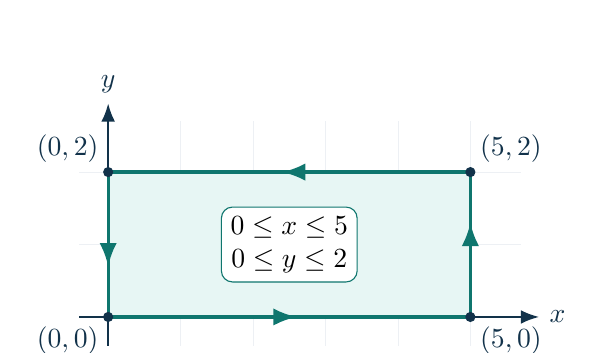
\begin{tikzpicture}[scale=0.92, >=Latex]
  \draw[step=1, gridgray!35, very thin] (-0.4,-0.4) grid (5.7,2.7);
  \draw[->, navy, thick] (-0.4,0) -- (5.95,0) node[right] {$x$};
  \draw[->, navy, thick] (0,-0.4) -- (0,2.95) node[above] {$y$};
  \fill[softteal] (0,0) rectangle (5,2);
  \draw[teal, very thick, ->] (0,0) -- (2.6,0);
  \draw[teal, very thick] (0,0) -- (5,0);
  \draw[teal, very thick, ->] (5,0) -- (5,1.3);
  \draw[teal, very thick] (5,0) -- (5,2);
  \draw[teal, very thick, ->] (5,2) -- (2.4,2);
  \draw[teal, very thick] (5,2) -- (0,2);
  \draw[teal, very thick, ->] (0,2) -- (0,0.7);
  \draw[teal, very thick] (0,2) -- (0,0);
  \fill[navy] (0,0) circle (2pt) node[below left] {$(0,0)$};
  \fill[navy] (5,0) circle (2pt) node[below right] {$(5,0)$};
  \fill[navy] (5,2) circle (2pt) node[above right] {$(5,2)$};
  \fill[navy] (0,2) circle (2pt) node[above left] {$(0,2)$};
  \node[align=center, fill=white, draw=teal, rounded corners] at (2.5,1.0)
  {$0\le x\le5$\\$0\le y\le2$};
\end{tikzpicture}
\caption{The rectangle has constant limits in both variables.}
\end{figure}

\begin{reasonbox}{Step 1: Identify \(P\) and \(Q\)}
Here
\[
P(x,y)=\cos y,
\qquad
Q(x,y)=x^2\sin y.
\]
\end{reasonbox}

\begin{reasonbox}{Step 2: Compute Green's Theorem integrand}
Compute
\[
\pd{Q}{x}=\pd{}{x}(x^2\sin y)=2x\sin y.
\]
Compute
\[
\pd{P}{y}=\pd{}{y}(\cos y)=-\sin y.
\]
Therefore
\[
\pd{Q}{x}-\pd{P}{y}=2x\sin y-(-\sin y)=(2x+1)\sin y.
\]
\end{reasonbox}

\begin{reasonbox}{Step 3: Set up the double integral}
The rectangular region is
\[
0\le x\le5,
\qquad
0\le y\le2.
\]
Therefore Green's Theorem gives
\[
\oint_C \cos y\,dx+x^2\sin y\,dy
=\int_0^5\int_0^2(2x+1)\sin y\,dy\,dx.
\]
\end{reasonbox}

\begin{reasonbox}{Step 4: Evaluate explicitly}
Because \(2x+1\) is constant with respect to \(y\),
\[
\int_0^2(2x+1)\sin y\,dy=(2x+1)\int_0^2\sin y\,dy.
\]
Now
\[
\int \sin y\,dy=-\cos y.
\]
Thus
\[
\int_0^2\sin y\,dy=[-\cos y]_0^2=-\cos2-(-\cos0)=1-\cos2.
\]
So the full integral becomes
\[
\int_0^5(2x+1)(1-\cos2)\,dx.
\]
The factor \((1-\cos2)\) is constant with respect to \(x\), so
\[
\int_0^5(2x+1)(1-\cos2)\,dx=(1-\cos2)\int_0^5(2x+1)\,dx.
\]
Now
\[
\int(2x+1)\,dx=x^2+x.
\]
Therefore
\[
\int_0^5(2x+1)\,dx=[x^2+x]_0^5=(25+5)-0=30.
\]
Hence
\[
\oint_C \cos y\,dx+x^2\sin y\,dy=30(1-\cos2).
\]
\end{reasonbox}

\begin{answerbox}
\[
\boxed{\oint_C \cos y\,dx+x^2\sin y\,dy=30(1-\cos2).}
\]
\end{answerbox}

\newpage
\subsection{Problem 3(iii): Circle of radius \texorpdfstring{\(a\)}{a}}
Evaluate
\[
\oint_C x\,dy-y\,dx,
\]
where \(C\) is the positively oriented circle of radius \(a\).

\begin{figure}[H]
\centering
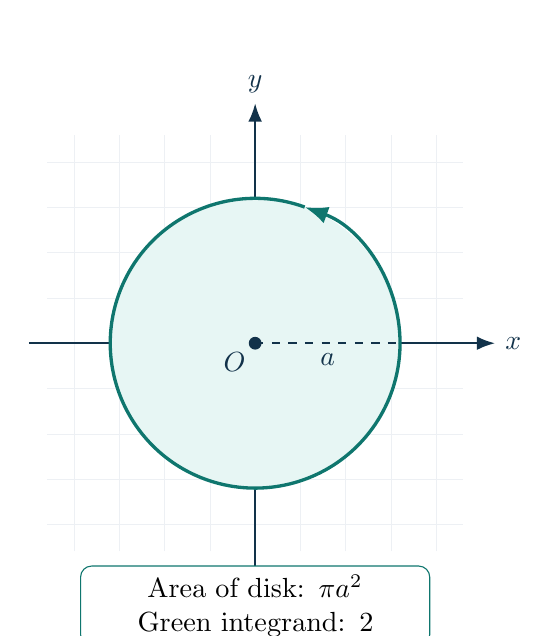
\begin{tikzpicture}[scale=1.15, >=Latex]
  \draw[step=0.5, gridgray!35, very thin] (-2.3,-2.3) grid (2.3,2.3);
  \draw[->, navy, thick] (-2.5,0) -- (2.65,0) node[right] {$x$};
  \draw[->, navy, thick] (0,-2.5) -- (0,2.65) node[above] {$y$};
  \fill[softteal] (0,0) circle (1.6);
  \draw[teal, very thick, ->] (1.6,0) arc (0:70:1.6);
  \draw[teal, very thick] (70:1.6) arc (70:360:1.6);
  \draw[dashed, navy, thick] (0,0) -- (1.6,0) node[midway, below] {$a$};
  \fill[navy] (0,0) circle (2pt) node[below left] {$O$};
  \node[align=center, fill=white, draw=teal, rounded corners, text width=4.2cm] at (0,-2.9)
  {Area of disk: $\pi a^2$\\Green integrand: $2$};
\end{tikzpicture}
\caption{Green's Theorem converts the boundary integral into twice the area of the disk.}
\end{figure}

\begin{reasonbox}{Step 1: Put the integral in Green's Theorem form}
The integral is
\[
\oint_C x\,dy-y\,dx.
\]
Write it as
\[
\oint_C P\,dx+Q\,dy.
\]
The coefficient of \(dx\) is \(-y\), and the coefficient of \(dy\) is \(x\). Therefore
\[
P(x,y)=-y,
\qquad
Q(x,y)=x.
\]
\end{reasonbox}

\begin{reasonbox}{Step 2: Compute Green's Theorem integrand}
Compute
\[
\pd{Q}{x}=\pd{}{x}(x)=1.
\]
Compute
\[
\pd{P}{y}=\pd{}{y}(-y)=-1.
\]
Therefore
\[
\pd{Q}{x}-\pd{P}{y}=1-(-1)=2.
\]
\end{reasonbox}

\begin{reasonbox}{Step 3: Convert to an area integral}
By Green's Theorem,
\[
\oint_C x\,dy-y\,dx=\iint_R 2\,dA,
\]
where \(R\) is the disk of radius \(a\).  Since
\[
\iint_R 1\,dA=\operatorname{Area}(R)=\pi a^2,
\]
we get
\[
\iint_R 2\,dA=2\iint_R 1\,dA=2\pi a^2.
\]
\end{reasonbox}

\begin{answerbox}
\[
\boxed{\oint_C x\,dy-y\,dx=2\pi a^2.}
\]
\end{answerbox}

\section{Final answer summary}

\begin{center}
\renewcommand{\arraystretch}{1.35}
\begin{tabular}{>{\raggedright\arraybackslash}p{0.28\textwidth} >{\raggedright\arraybackslash}p{0.58\textwidth}}
\toprule
\textbf{Problem} & \textbf{Final result}\\
\midrule
1(i) & Independent of path; value \(\displaystyle \frac{4}{e}\).\\
1(ii) & Independent of path; value \(\displaystyle -2\).\\
2(i) & Circle of radius \(1\): value \(\displaystyle 2\pi\).\\
2(ii) & Circle of radius \(2\): value \(\displaystyle 2\pi\).\\
3(i) & Triangle integral: \(\displaystyle 12\).\\
3(ii) & Rectangle integral: \(\displaystyle 30(1-\cos2)\).\\
3(iii) & Circle of radius \(a\): \(\displaystyle 2\pi a^2\).\\
\bottomrule
\end{tabular}
\end{center}

\end{document}
